\chapter{Continuous gravitational wave injections}

%%%%%%%%%%%%%%%%
In this section I outline how we inject a \gls{CW} signal into data. This can generally be done in two different ways: simulating a signal in the time domain and injecting into time domain noise or simulating the signal in the frequency domain. 
The searches described in Sec.~\ref{soap} and Sec.~\ref{cnn} only use output power spectra] 
Generating the time series and performing a Fourier transform or generating the signal in the frequency domain is time consuming. 
In this section I will outline how I simulate the power spectrum of \gls{CW} signals and inject them into a \gls{PSD}.
This should greatly improve the speed of data generation.


%%%%%%%%%%%%%%%
\section{Signal SNR}
%%%%%%%%%%%%%

To inject into a spectrogram the power spectrum of the signal will need to be simulated. In our injection we do not have access to a time-series, therefore, we do not simulate the signal in in the time series or complex frequency domain. 
Instead, the \gls{SNR} of the signal can be estimated in given frequency bins and injected straight into the power spectrum.

It can be shown that the \gls{PSD} of Gaussian noise with zero mean and unit variance is a $\chi^2$ distribution with 2 degrees of freedom. Therefore, if we want to generate a spectrogram for Gaussian noise, we just generate a two dimensional array of values distributed as $\chi^2$ with two degrees of freedom.
Assuming that there is some sinusoidal signal with a given \gls{SNR} within a Gaussian noise time-series with zero mean and unit variance, the \gls{FFT} power in a particular frequency bin can be estimated using a non-central $\chi^2$ distribution with 2 degrees of freedom, where the non centrality parameter is the square of the \gls{SNR}. 
To calculate the \gls{SNR} in a given frequency bin the equation in \citep{prix2007SearchContinuous} for optimal \gls{SNR} was used,
\begin{equation}
	\label{app1:snr2}
    \rho(0)^2 = \frac{1}{2}h_0^2 T S^{-1} \left[ \alpha_1 A + \alpha_2 B + \alpha_3 C \right],
\end{equation}
where $h_0$ is the \gls{GW} amplitude, $T$ is the total observing time is seconds, $S^{-1}$ is the mean \gls{PSD} noise floor. The values of $\alpha$ are then defined in \citep{prix2007SearchContinuous} by,
\begin{equation}
\begin{split}
\alpha_1 &= \frac{1}{4}\left(1 + \cos^2 \left( \iota\right)  \right)^2 \cos^2\left( 2 \psi \right)  + \cos^2\left( \iota\right)  \sin^2 \left( 2\psi \right) \\
\alpha_2 &= \frac{1}{4}\left(1 + \cos^2 \left( \iota \right) \right)^2 \sin^2\left( 2 \psi \right)  + \cos^2\left( \iota\right)  \cos^2 \left( 2\psi \right) \\
\alpha_3 &= \frac{1}{4}\left(1 - \cos^2 \left( \iota\right)  \right)^2 \sin\left( 2 \psi \right) \sin^2 \left( 2\psi \right) \\
\end{split}
\end{equation}
where $\psi$ is the gravitational wave phase and $\iota$ is the inclination angle of the source.
The values of $A,B$ and $C$ in Eq.~\ref{app1:snr2} are functions which represent the time averages antenna patterns, they are defined by,
\begin{equation}
\begin{split}
A &\equiv \langle a^2 \rangle \\
B &\equiv \langle b^2 \rangle \\
C &\equiv \langle ab \rangle, \\
\end{split}
\end{equation}
where $a$ and $b$ are the antenna pattern functions defined in \citep{schutz1998DataAnalysis} as,
\begin{equation}
\begin{split}
a(t) &= \frac{1}{16}\sin{2\gamma}(3-\cos{2\lambda})(3-\cos2\delta)\cos[2(\alpha-\phi_r -\Omega t)] \\
&- \frac{1}{4}\cos{2\gamma}\sin\lambda(3-\cos2\delta)\sin[2(\alpha-\phi_r -\Omega t)] \\
&+ \frac{1}{4}\sin{2\gamma}\sin2\lambda\sin2\delta\cos[\alpha-\phi_r -\Omega t] \\
&- \frac{1}{2}\cos{2\gamma}\cos{\lambda}\sin{2\delta}\sin[\alpha-\phi_r -\Omega t] \\
&+ \frac{3}{4}\sin{2\gamma}\cos^2{\lambda}\cos^2{\delta} ,\\
\\
b(t) &= \cos{2\gamma}\sin{\lambda}\sin{\delta}\cos[2(\alpha-\phi_r -\Omega t)] \\
&+ \frac{1}{4}\sin{2\gamma}(3-\cos2\lambda)\sin{\delta}\sin[\alpha-\phi_r -\Omega t] \\
&+ \cos{2\gamma}\cos{\lambda}\cos{\delta}\cos[\alpha-\phi_r -\Omega t] \\
&+ \frac{1}{4}\sin{2\gamma}\sin{2\lambda}\cos{\delta}\sin[\alpha-\phi_r -\Omega t] .\\
\end{split}
\end{equation}
Here$\gamma$ is the orientation of the detectors arms, $\lambda$ is the latitude of the detectors site, $\alpha$ and $\delta$ are the right ascension and declination of the \gls{GW}, $\phi_r$ is a deterministic phase defining the position of the earth and $\Omega$ is the rotational angular velocity of the earth.
This takes into account the antenna pattern modulation of the signal as the earth rotates the sun and orbits the earth.
We then have a description of the \gls{SNR} of a signal with a set of parameters for any given time and duration. 
This however does not describe how the \gls{SNR} of a signal varies with frequency which we need for spectrogram injections.

%%%%%%5
%%%%%%
\section{SNR with frequency}
%%%%%%
%%%%%%

If one takes a sinusoidal signal and the takes the Fourier transform of that, then this should be a delta function at the frequency of the sinusoid. 
However, in the real world this sinusoid has a limited length and one will instead take the \gls{FFT} of that signal, the signal will then be broken into discrete frequency bins.
If the sinusoids frequency falls at the center of a frequency bin then the entire power of the signal will be contained within that frequency bin.
However, if it is not perfectly centered on a frequency bin, then the power of the signal will begin to be spread over surrounding frequency bins. 
The aim is then to simulate how the signal is spread over surrounding frequency bins.
If one has a sinusoid with a finite length, this is equivalent to taking an infinitely long sinusoid and convolving it square window (box). 
The frequency response is then the Fourier transform of the sinusoid convolved with the Fourier transform of the box window.
The Fourier transform of a box window is a sinc and of an infinitely long sinusoid is a delta function. 
The resulting Fourier transform is then a sinc function.
One can show this by taking the power spectrum of a finite length sinusoid, and plotting the square of a sinc function on top as shown in Fig.~\ref{app1:sin:sinc}.

\begin{figure}
	\centering
	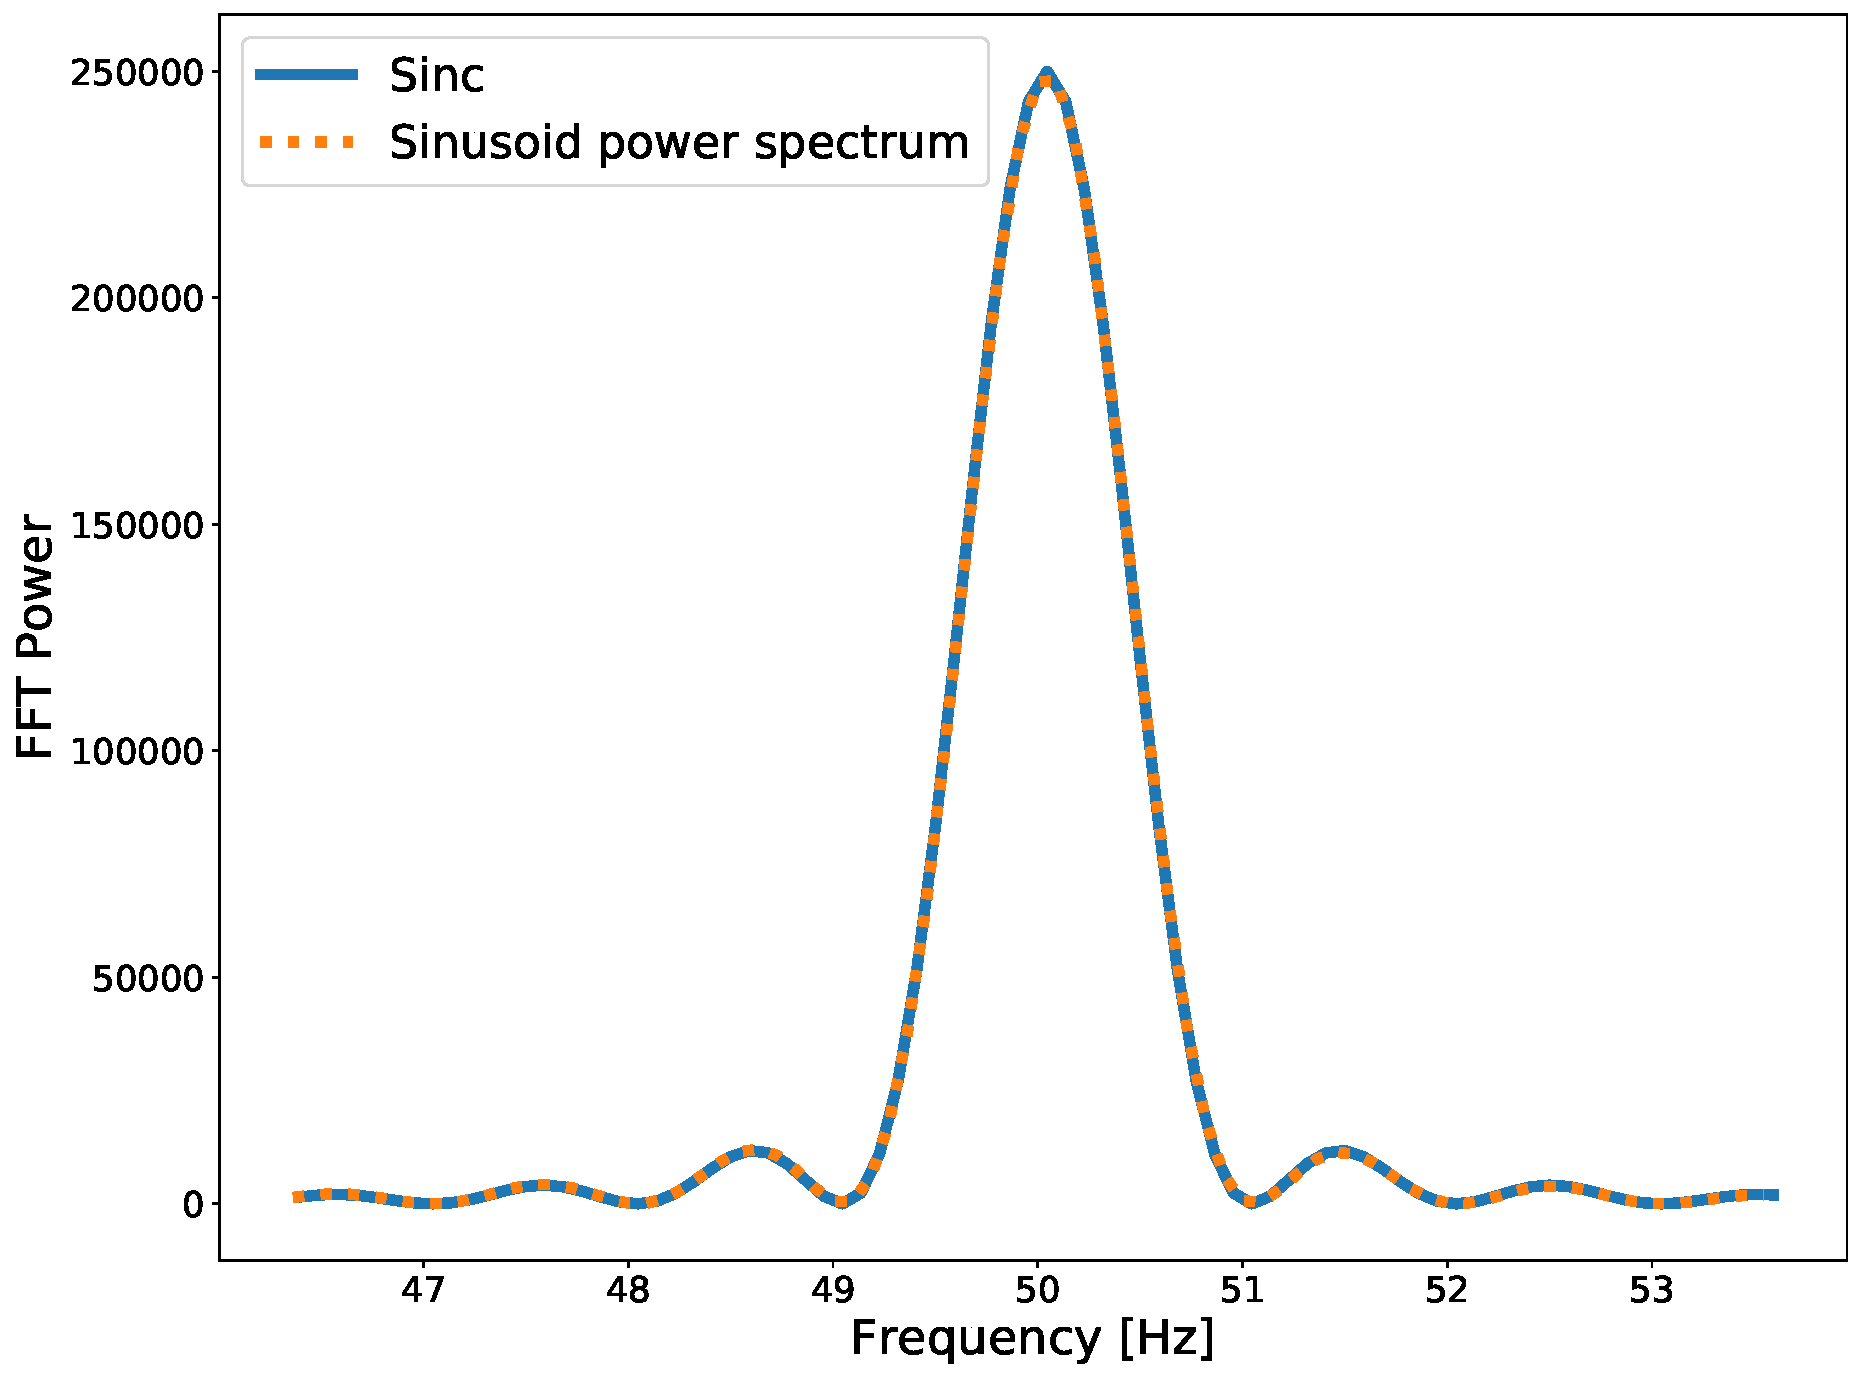
\includegraphics[width=0.7\linewidth]{AppendixA/sinc_fft.pdf}
	\caption[Sinc function compared to \gls{FFT} of finite length sinusoid.]{If one takes the power spectrum of a sinusoid with finite length, this returns the same distribution as the square of a sinc function.}
	\label{app1:sin:sinc}
\end{figure}

For a sinusoid which has some frequency derivative the Fourier transform changes slightly. 
One can start with the definition of a signal with a constant frequency derivative, 
\begin{equation}
n(t) = a \cos{\left[2\pi (f_0 t + 1/2 \dot{f} t^2) + \phi \right]},
\end{equation}
where $f$ is its frequency, $\dot{f}$ is its frequent derivative and $t$ is time.
In cases that follow we will have a finite frequency length, therefore when computing the Fourier transform, this is equivalent to applying a box window the signal.
If we define the length of our signal as $T$ we can redefine some terms as,
\begin{equation}
\begin{split}
u &= \frac{t}{T} \\
r &= f T \\
\dot{r} &= \dot{f} T^2 .\\
\end{split}
\end{equation}
The signal can now be written in terms of $u$ and $r$ as,
\begin{equation}
\begin{split}
n(u) &= a \cos{\left[2\pi (r_0 u + 1/2 \dot{r} u^2) + \phi\right]} \\
&= \frac{1}{2} a \left[ e^{i 2\pi(r_0 u + 1/2 \dot{r} u^2)}e^{i\phi}  + e^{-i 2\pi(r_0 u + 1/2 \dot{r} u^2)}e^{-i\phi}    \right] \\
\end{split}
\end{equation}
As the signal is zero outside of $0 \leq u \leq	 1$, as in \citep{ransom2002FourierTechniques} we can write the Fourier transform at some frequency $r_c$ as,
\begin{equation}
\begin{split}
\tilde{n}(r_c) &= \frac{aN}{2}  \int_{0}^{1} n(u) \exp{\left\{ -i 2 \pi u r_c\right\}} du \\
&= \frac{aN}{2} \left[ e^{i\phi} \int_{0}^{1} e^{i 2 \pi(\frac{\dot{r}}{2} u^2 + r_{0c}u - r_cu)} du  +  e^{-i\phi}\int_{0}^{1} e^{-i 2 \pi(\frac{\dot{r}}{2} u^2 + r_{0c}u + r_cu)} du\right] \\
&= \frac{aN}{2} e^{i\phi} \left[  I_1 + I_2   \right], \\
\end{split}
\end{equation}
where $r_c = r + \dot{r}/2$ and the signal frequency at bin center is $r_{0c} = r_0 + \dot{r}/2$.
The first integral can then be written as,
\begin{equation}
\begin{split}
I_1 &= \int_{0}^{1} \exp{\left\{i 2 \pi(\frac{\dot{r}}{2} u^2 + r_{0c}u - r_cu) \right\}} du \\
&= \int_{0}^{1} \exp{\left\{ i 2 \pi\left(\frac{\dot{r}}{2} u^2 + (r_{0c} - r_c)u \right) \right\}} du \\
& = \int_{0}^{1} \exp{\left\{i \frac{\pi}{2} 2 \dot{r} \left(u^2 + 2\frac{(r_{0c} - r_c)}{\dot{r}}u \right)\right\}} du \\
& = \int_{0}^{1} \exp{\left\{i \frac{\pi}{2} 2 \dot{r} \left[\left(u + \frac{(r_{0c} - r_c)}{\dot{r}} \right)^2 - \left(\frac{(r_{0c} - r_c)}{\dot{r}}\right)^2 \right]\right\}} du \\
& = \exp{\left\{  - i \frac{\pi}{2} 2 \dot{r} \left(\frac{(r_{0c} - r_c)}{\dot{r}}\right)^2 \right\}}\int_{0}^{1} \exp{\left\{i \frac{\pi}{2} 2 \dot{r} \left[\left(u + \frac{(r_{0c} - r_c)}{\dot{r}} \right)^2 \right]\right\}} du \\
\end{split}
\end{equation}
We can then substitute using,
\begin{equation}
v = \sqrt{2\dot{r}}\left( u + \frac{(r_{0c} - r_c)}{\dot{r}}  \right)
\end{equation}
where,
\begin{equation}
dv = \sqrt{2\dot{r}} du 
\end{equation}
and when $u = 1$ we can define $Y$ as,
\begin{equation}
Y = \sqrt{2\dot{r}}\left( 1 + \frac{(r_{0c} - r_c)}{\dot{r}}  \right)
\end{equation}
The integral then becomes,
\begin{equation}
\begin{split}
I_1 & = \exp{\left\{  - i \frac{\pi}{2} 2 \dot{r} \left(\frac{(r_{0c} - r_c)}{\dot{r}}\right)^2 \right\}} \sqrt{2\dot{r}}  \int_{0}^{Y} \exp{\left\{i \frac{\pi}{2} v^2\right\}} dv \\
& = \exp{\left\{  - i \frac{\pi}{2} 2 \dot{r} \left(\frac{(r_{0c} - r_c)}{\dot{r}}\right)^2 \right\}} \sqrt{2\dot{r}}  \int_{0}^{Y} 
\cos{\left(  \frac{\pi}{2} v^2 \right)} + i\sin{\left(  \frac{\pi}{2} v^2 \right)} dv \\
\end{split}
\end{equation}
Similarly, using,
\begin{equation}
Z = \sqrt{2\dot{r}}\left( 1 - \frac{(r_{0c} - r_c)}{\dot{r}}  \right)
\end{equation}
one can write,
\begin{equation}
\begin{split}
I_2 & = \exp{\left\{  - i \frac{\pi}{2} 2 \dot{r} \left(\frac{(r_{0c} - r_c)}{\dot{r}}\right)^2 \right\}} \sqrt{2\dot{r}}  \int_{0}^{Z} \exp{\left\{i \frac{\pi}{2} v^2\right\}} dv \\
& = \exp{\left\{  - i \frac{\pi}{2} 2 \dot{r} \left(\frac{(r_{0c} - r_c)}{\dot{r}}\right)^2 \right\}} \sqrt{2\dot{r}}  \int_{0}^{Z} 
\cos{\left(  \frac{\pi}{2} v^2 \right)} + i\sin{\left(  \frac{\pi}{2} v^2 \right)} dv \\
\end{split}
\end{equation}

One can then use the Fresnel $S(x)$ and $C(x)$ defined by
\begin{equation}
\begin{split}
C(x) &= \int_0^x \cos{\frac{\pi}{2} t^2} dt \\
S(x) &= \int_0^x \sin{\frac{\pi}{2} t^2} dt \\
\end{split}
\end{equation}
The Fourier transform is then,
\begin{equation}
A_{r_c} = \frac{aN}{2\sqrt{2\dot{r}}} e^{i(\phi - \pi q^2/\dot{r})} \left[ S(Z) -  S(Y) + i(C(Y) - C(Z))   \right],
\end{equation}
where,
The power spectrum is then
\begin{equation}
|A_{r_c}|^2 = \frac{a^2 N^2}{4\dot{r}}  \left[ (S(Z) -  S(Y))^2 + (C(Y) - C(Z))^2   \right]
\end{equation}

This can then be converted back into frequencies using the relations in Eq.~\ref{},
\begin{equation}
\label{app1:power_fresnel}
|A_{r_c}|^2 = \frac{a^2 N^2}{4\dot{f}T^2}  \left[ (S(Z) -  S(Y))^2 + (C(Y) - C(Z))^2   \right]
\end{equation}
and,
\begin{equation}
\begin{split}
Z &= \sqrt{2\dot{f}}T\left( 1 - \frac{(f_{0c} - f_c)}{\dot{f}T}  \right) \\
Y &= \sqrt{2\dot{f}}T\left( 1 + \frac{(f_{0c} - f_c)}{\dot{f}T}  \right) \\
\end{split}
\end{equation}
\joe{there is a factor of 2 missing and its annoying $2\frac{(f_{0c} - f_c)}{\dot{f}T}$}

By taking a simple signal, we can verify that this is correct. Fig.~\ref{app1:sinderivative:fresnel} demonstrates the \gls{FFT} of a simple signal and the power spectrum estimation using Eq.~\ref{app1:power_fresnel}.

\begin{figure}
	\centering
	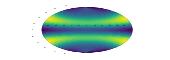
\includegraphics[width=\linewidth]{testimg.png}
	\caption[Comparison of power spectrum simulation with \gls{FFT} of sinusoid with frequency derivative.]{comparing sin fft with sinc function}
	\label{app1:sinderivative:fresnel}
\end{figure}

The values of this for the center location of each frequency bin surrounding the signal frequency can then be calculated for each time segment. 
A full spectrogram of a loud signal ($\sim 1000$ \gls{SNR}) can be seen in Fig.~\ref{app1:spect:centerbin}, \ref{app1:spect:edgebin}, \ref{app1:spect:doppler} and \ref{app1:spect:antenna} to demonstrate the signal simulations.
The signal frequency for each time segment can be found using the model described in Sec.~\ref{searchcw:model}.
Fig.~\ref{app1:spect:centerbin} shows an example of a signal of fixed frequency which is simulated at the center of a frequency bin.
\begin{figure}[h]
	\centering
	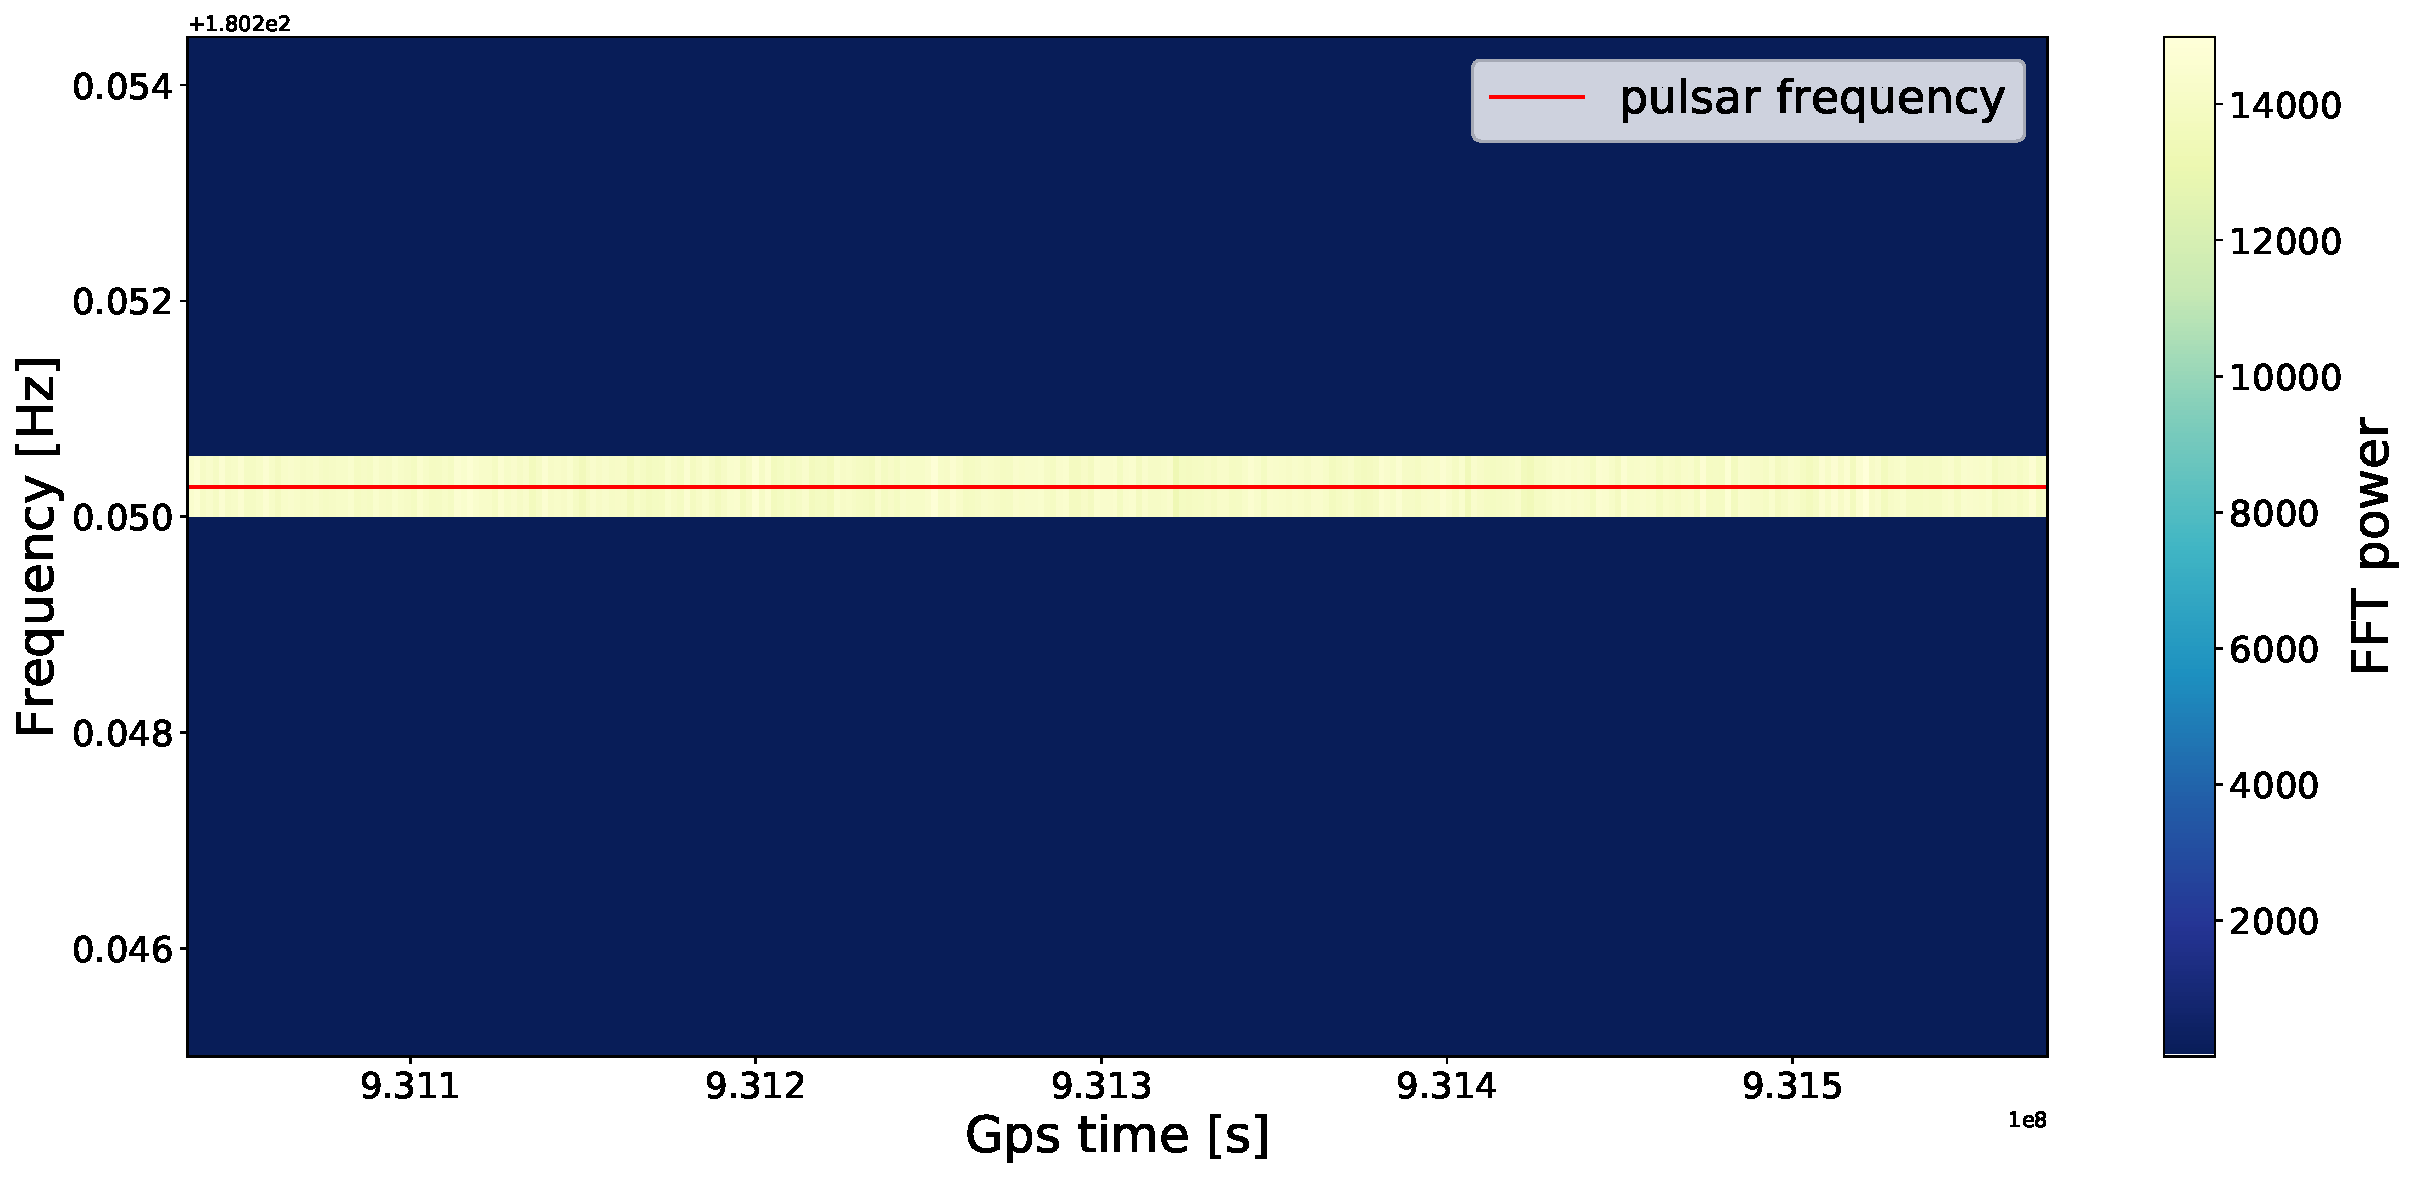
\includegraphics[width=\linewidth]{AppendixA/centerbin_nodop_noant.pdf}
	\caption[Generated spectrogram in center of frequency bin.]{By simulating a signal with a frequency in the center of a band, all of the signals power is contained within a single frequency bin. This shows an example of this kind of simulation in a spectrogram. The red line is the signals frequency evolution.}
	\label{app1:spect:centerbin}
\end{figure}
When the signals frequency is then moved to the edge of a bin, the power can be seen to be distributed evenly between the two surrounding frequency bins. This can be seen in Fig.~\ref{app1:spect:edgebin}.
\begin{figure}[h]
	\centering
	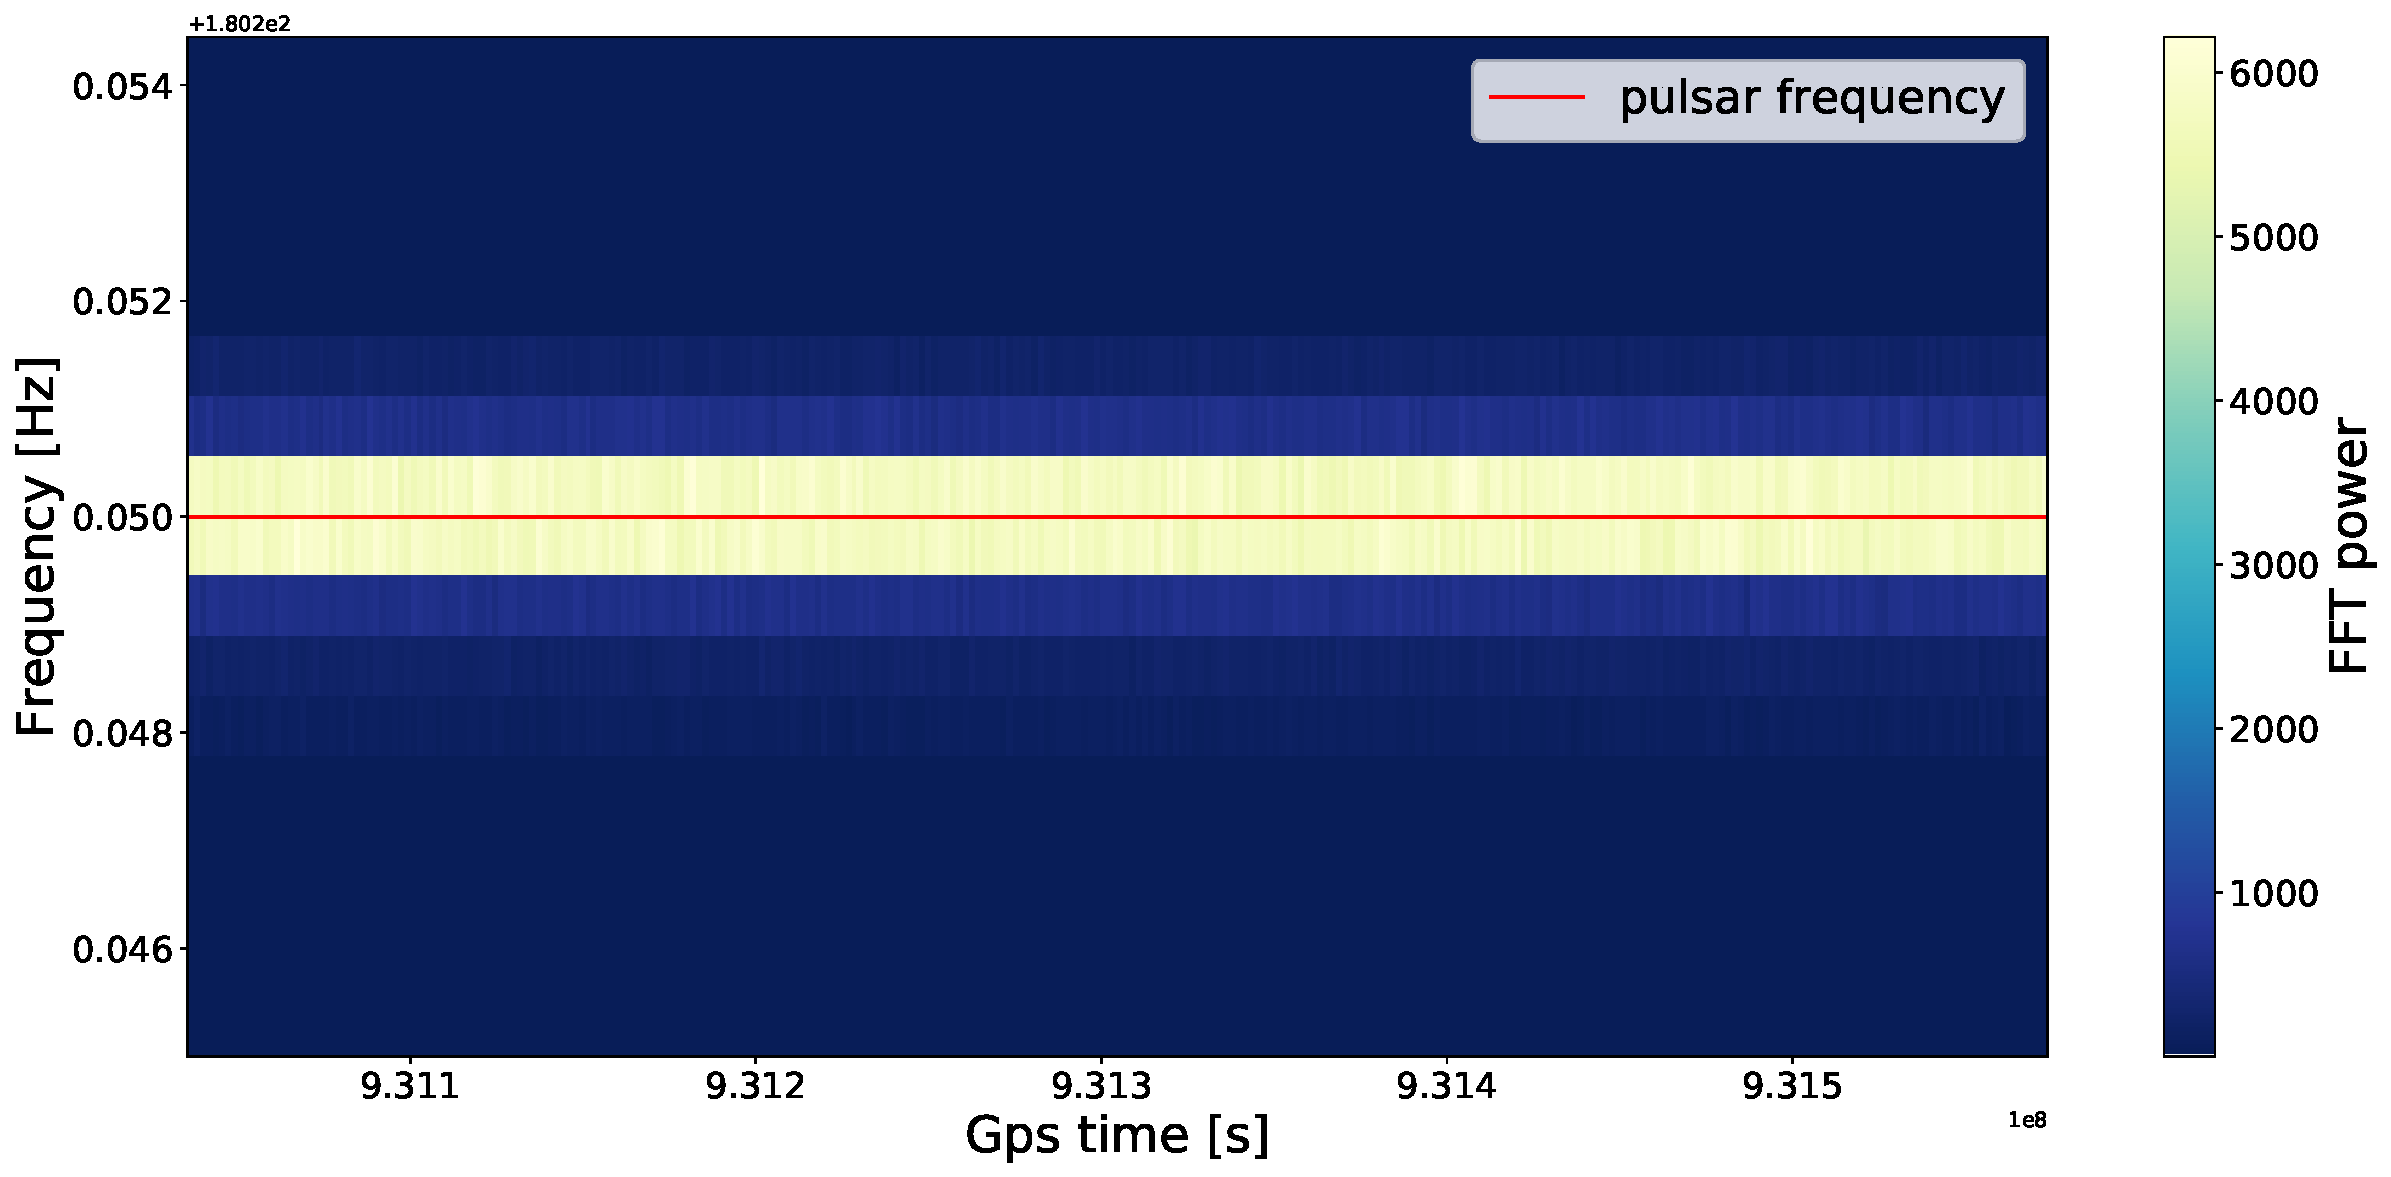
\includegraphics[width=\linewidth]{AppendixA/edgebin_nodop_noant.pdf}
	\caption[Generated spectrogram at edge of frequency bin.]{By placing the signal at the edge of a frequency bin, the power is distributed around surrounding frequency bin, this can be seen above. The red line is the signals frequency evolution.}
	\label{app1:spect:edgebin}
\end{figure}
The doppler shift of a signal can then be added such that the frequency changes with time. This is shown in Fig.~\ref{app1:spect:doppler}.
\begin{figure}[h]
	\centering
	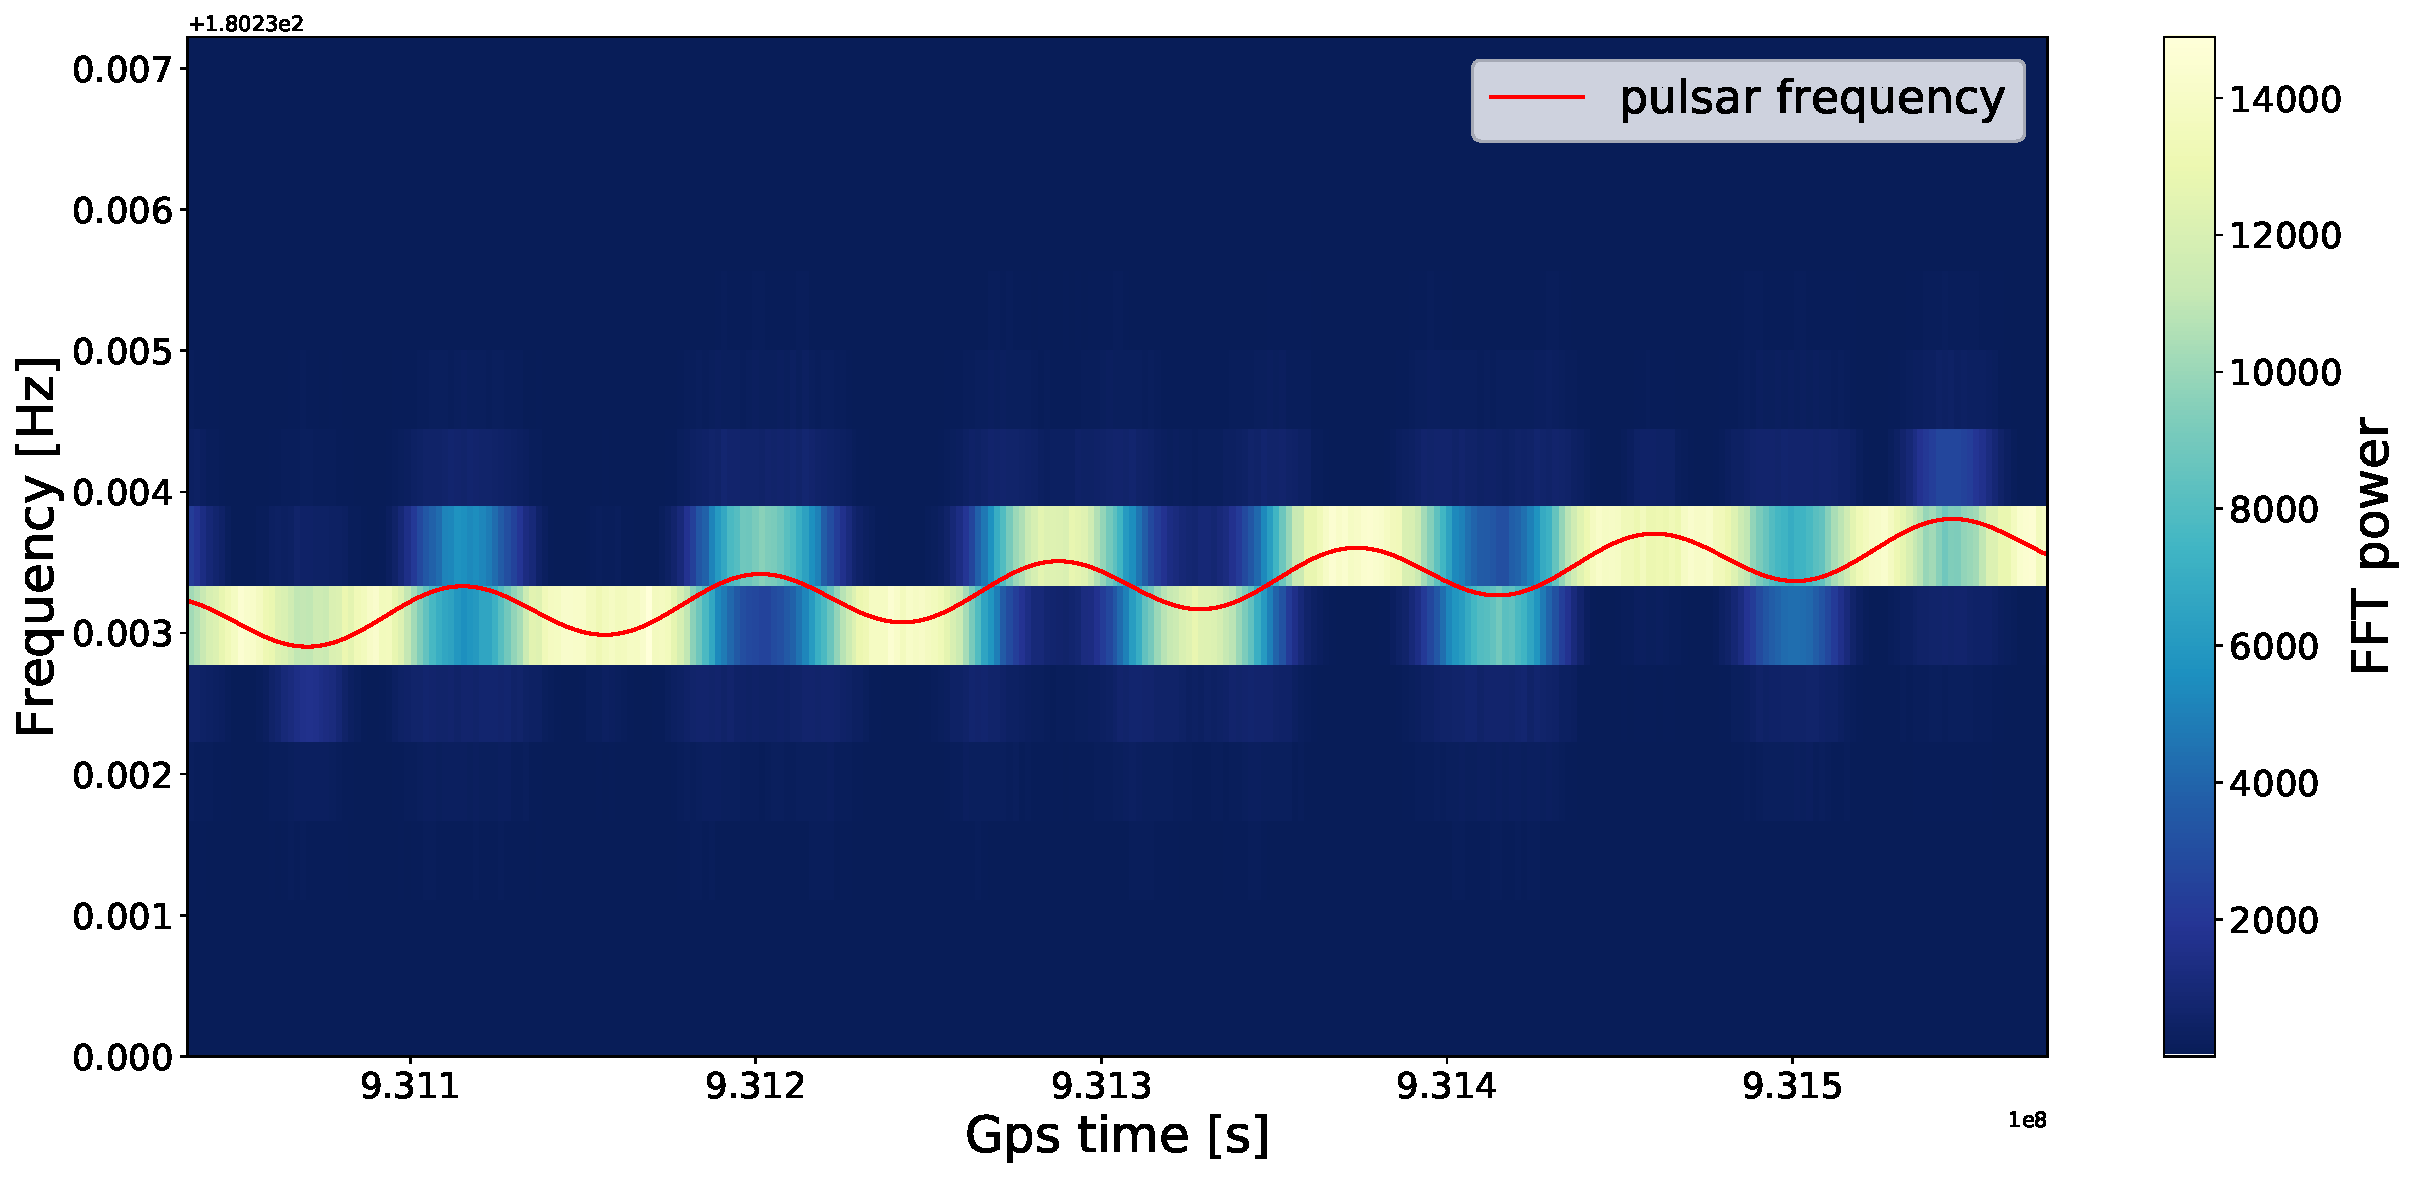
\includegraphics[width=\linewidth]{AppendixA/edgebin_doppler_noant.pdf}
	\caption[Generated spectrogram of \gls{CW} signal with Doppler shift.]{Including the Doppler shift of a signal due to the earths rotation and orbit cause the signal to be modulated in frequency. This also causes a modulation in the \gls{SNR} of the signal in and single frequency bin as it moves between bins. The red line is the signals frequency evolution.}
	\label{app1:spect:doppler}
\end{figure}
Finally Fig.~\ref{app1:spect:antenna} shows the Doppler modulation and the antenna pattern modulation of a \gls{CW} signal. 
\begin{figure}[h]
	\centering
	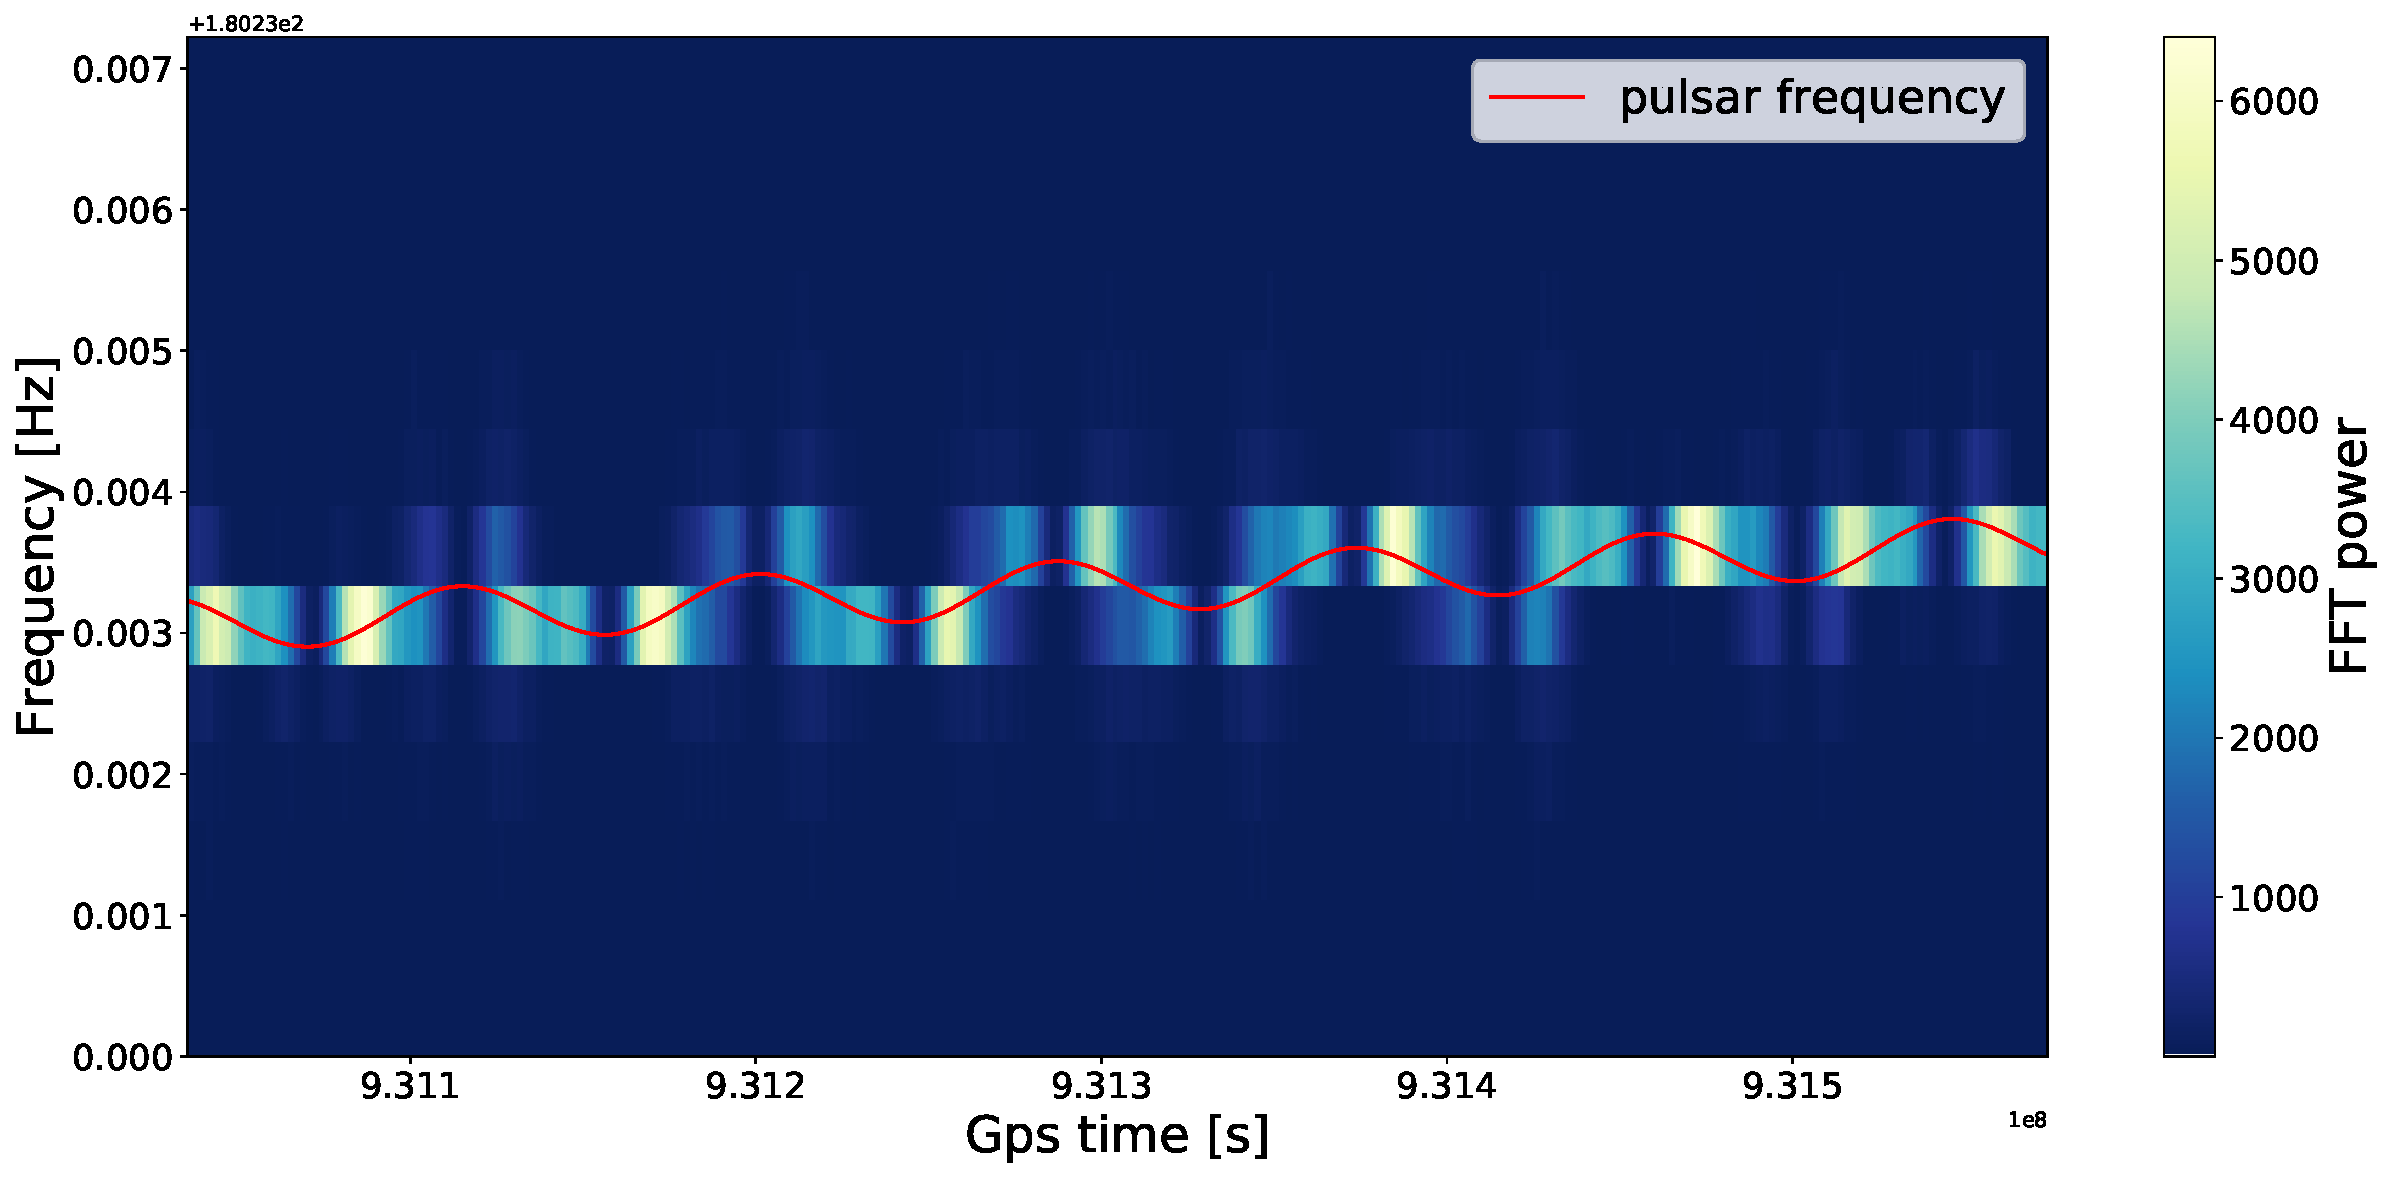
\includegraphics[width=\linewidth]{AppendixA/edgebin_doppler_antenna.pdf}
	\caption[Generated spectrogram of \gls{CW} signal with Doppler shift and antenna pattern modulation.]{The antenna pattern modulation can also be included to completely simulate a potential \gls{CW} signal in a spectrogram. The red line is the signals frequency evolution.}
	\label{app1:spect:antenna}
\end{figure}

These simulations in the power spectrum greatly increased the speed of data generation when compared to simulating the signal in the time-series and taking their Fourier transform.
